% todo:
% puddle algorithm: shorten it:
% graphics for slides
% ensure notation is consistent and comprehensive
%

\documentclass{beamer}
\usetheme{default}
\usepackage{shortcuts}
\usepackage{tikz}

\title[Abstract Pattern Formation]{A Randomized Approach to Abstract Pattern Formation Fat Robots}
%\subtitle[Errors]{Estimation of numerical errors}
\author[A. Diaz Tolentino \& S. Ramamoorthy]{Armando Jesus Diaz Tolentino \& Sivaramakrishnan Natarajan Ramamoorthy}
\institute[UW]{
	Department of Computer Science\\
	University of Washington\\
	Seattle, Washington \\[1ex]
	\texttt{\{ajdt, sivanr\}@cs.washington.edu}
}
\begin{document}

\begin{frame}
	\titlepage	
\end{frame}
\begin{frame}
	\tableofcontents
\end{frame}

% justify why the problem is cool, applications!!
\begin{frame}{Problem Introduction}
	\textbf{Arbitrary Pattern Formation (APF):} 
	\begin{itemize}
		\item Given: A set of $n$ robots arranged arbitrarily on 2D plane 
		\item Goal: form an arbitrary pattern known by all robots \textit{a priori}
		\item Operations: Look, Move, Wait
		\item No explicit communication between robots
	\end{itemize}

	Related Problems:
	\begin{itemize}
	% todo: insert graphics to make these problems clear
		\item gathering
		\item pattern sequencing
		\item flocking
	\end{itemize}
\end{frame}

% insert slide for motivations

\begin{frame}{Modelling Choices}
	Various Modelling Choices:
	\begin{itemize}
		\item history oblivious, synchronous (FSYNC), ansynchronous (ASYNC)
		\item point vs disk model, transparent vs opaque
	\end{itemize}

	Assumptions:
	\begin{itemize}
		\item compass orientations: 
		\begin{itemize}
			\item consistent compass
			\item OneAxis
			\item Chirality
		\end{itemize} 
		\item rescaling and rotation of shape
		\item number of robots
		% TODO
		<insert graphics here to explain concepts>
	\end{itemize}
\end{frame}

\begin{frame}{Notation}
	\begin{itemize}
		\item We refer to a configuration, $\EE$, as an $n$-tuple of points: $\EE = (x_1,\ldots x_n)$, $x_i \in \RR^2$
		\item $\EE_i$ is configuration seen by robot $i$
		\item $\PP$ target pattern robots must form
		\item global view and local view definitions HERE!! % TODO
	\end{itemize}
\end{frame}

\begin{frame}{Prior Work: Impossibility Results}
	\begin{theorem} 
		APF is not solvable deterministically for an even number of robots $ n > 2$.
	\end{theorem} 
	%\begin{float}[H]
		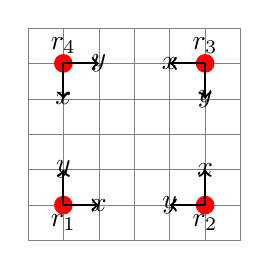
\begin{tikzpicture}[scale=0.45]
			\draw[help lines] (0,0) grid (6,6);

			% circles
			\draw [red, fill, ultra thick] (1,1) circle [radius=0.2];;
			\draw [red, fill, ultra thick] (5,1) circle [radius=0.2];;
			\draw [red, fill, ultra thick] (5,5) circle [radius=0.2];;
			\draw [red, fill, ultra thick] (1,5) circle [radius=0.2];;

			% axes
			\draw[thick, ->] (1,1) -- (1,2) ; % robot 1
			\draw[thick, ->] (1,1) -- (2,1) ; 
			\node at (1,2) {$y$} ;
			\node at (2,1) {$x$} ;
			\draw[thick, ->] (5,1) -- (4,1) ; % robot 2
			\draw[thick, ->] (5,1) -- (5,2) ; 
			\node at (4,1) {$y$} ;
			\node at (5,2) {$x$} ;
			\draw[thick, ->] (5,5) -- (5,4) ; % robot 3
			\draw[thick, ->] (5,5) -- (4,5) ; 
			\node at (5,4) {$y$} ;
			\node at (4,5) {$x$} ;
			\draw[thick, ->] (1,5) -- (2,5) ; % robot 4
			\draw[thick, ->] (1,5) -- (1,4) ; 
			\node at (2,5) {$y$} ;
			\node at (1,4) {$x$} ;

			%\node[red, circle, minimum size=0.1cm] at (1,1) {$r_1$} ;
			\node[below] at (1,1) {$r_1$} ;
			\node[below] at (5,1) {$r_2$} ;
			\node[above] at (5,5) {$r_3$} ;
			\node[above] at (1,5) {$r_4$} ;

			% draw circles at positions desired
			%\draw [red, ultra thick] (0,0)
			%\draw (1,1) -- (5,1) -- (5,5) -- (1,5) -- (1,1);
		\end{tikzpicture}
	%\end{float}
	\begin{theorem} 
		APF is solvable deterministically for odd number of robots even in ASYNC.
	\end{theorem} 
		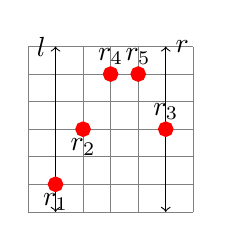
\begin{tikzpicture}[scale=0.35]
			\draw[help lines] (0,0) grid (6,6);

			\draw [<->] (1,0) -- (1,6) ;
			\draw [<->] (5,0) -- (5,6) ;
			% circles
			\draw [red, fill, ultra thick] (1,1) circle [radius=0.2];;
			\draw [red, fill, ultra thick] (2,3) circle [radius=0.2];;
			\draw [red, fill, ultra thick] (5,3) circle [radius=0.2];;
			\draw [red, fill, ultra thick] (3,5) circle [radius=0.2];;
			\draw [red, fill, ultra thick] (4,5) circle [radius=0.2];;

			% node labels
			\node[below] at (1,1) {$r_1$} ;
			\node[below] at (2,3) {$r_2$} ;
			\node[above] at (5,3) {$r_3$} ;
			\node[above] at (3,5) {$r_4$} ;
			\node[above] at (4,5) {$r_5$} ;
			% line labels
			\node[left] at (1,6) {$l$} ;
			\node[right] at (5,6) {$r$} ;
		\end{tikzpicture}

\end{frame}

% todo: fit this on one slide!!
\begin{frame}{prev result part 2}
		% APF solved
		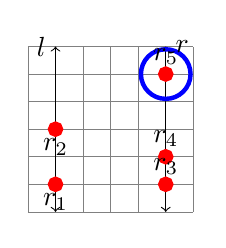
\begin{tikzpicture}[scale=0.35]
			\draw[help lines] (0,0) grid (6,6);

			\draw [<->] (1,0) -- (1,6) ;
			\draw [<->] (5,0) -- (5,6) ;
			% circles
			\draw [red, fill, ultra thick] (1,1) circle [radius=0.2];
			\draw [red, fill, ultra thick] (1,3) circle [radius=0.2];
			\draw [red, fill, ultra thick] (5,1) circle [radius=0.2];
			\draw [red, fill, ultra thick] (5,2) circle [radius=0.2];
			\draw [red, fill, ultra thick] (5,5) circle [radius=0.2];
			\draw [blue, ultra thick] (5,5) circle [radius=0.9]; % leader circle 

			% node labels
			\node[below] at (1,1) {$r_1$} ;
			\node[below] at (1,3) {$r_2$} ;
			\node[above] at (5,1) {$r_3$} ;
			\node[above] at (5,2) {$r_4$} ;
			\node[above] at (5,5) {$r_5$} ;

			% line labels
			\node[left] at (1,6) {$l$} ;
			\node[right] at (5,6) {$r$} ;
		\end{tikzpicture}
\end{frame}

\begin{frame}{Prior Work: APF and Leader Election}
	\begin{theorem} 
		APF is solvable for $n \geq 3$ robots $\iff$ Leader election problem is solvable.
	\end{theorem} 
	APF $\rightarrow$ leader election: \\
	\pause
	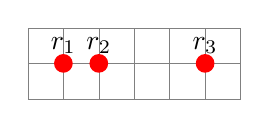
\begin{tikzpicture}[scale=0.45]
		\draw[help lines] (0,0) grid (6,2);
		% circles
		\draw [red, fill, ultra thick] (1,1) circle [radius=0.2];;
		\draw [red, fill, ultra thick] (2,1) circle [radius=0.2];;
		\draw [red, fill, ultra thick] (5,1) circle [radius=0.2];;

		%\node[red, circle, minimum size=0.1cm] at (1,1) {$r_1$} ;
		\node[above] at (1,1) {$r_1$} ;
		\node[above] at (2,1) {$r_2$} ;
		\node[above] at (5,1) {$r_3$} ;
	\end{tikzpicture}

	leader election $\rightarrow$ APF: \\
	\pause
	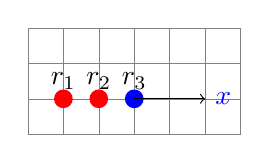
\begin{tikzpicture}[scale=0.45]
		\draw[help lines] (0,0) grid (6,3);
		% circles
		\draw [red, fill, ultra thick] (1,1) circle [radius=0.2];;
		\draw [red, fill, ultra thick] (2,1) circle [radius=0.2];;
		\draw [blue, fill, ultra thick] (3,1) circle [radius=0.2];;

		%\node[red, circle, minimum size=0.1cm] at (1,1) {$r_1$} ;
		\node[above] at (1,1) {$r_1$} ;
		\node[above] at (2,1) {$r_2$} ;
		\node[above] at (3,1) {$r_3$} ;

		% axis of agreement
		\draw [->] (3,1) -- (5,1) ;
		\node[right, blue, thick] at (5,1) {$x$} ;
	\end{tikzpicture}

	Using this insight, our algorithms work to solve leader election first.

\end{frame}

% insert description of puddle
% demonstrate how odd case works in previous algorithm???
\begin{frame}{Our Work: PUDDLE, a Randomized Approach}
	Our Model:
	\begin{itemize}
		\item unit disk, opaque, history oblivious, ASYNC
	\end{itemize}
	3 stages:
	\begin{enumerate}
		\item Move robots to vertical lines $l,r$
		\item If same number of robots on $l$ and on $r$, then break symmetry with randomness
		\item Elect leader from current configuration and form $\PP$
	\end{enumerate}
\end{frame}

\begin{frame}{PUDDLE: PART 1}
	\begin{enumerate}
		\item Compute vertical lines $l,r$ tangent to the convex hull of $\EE$, 
		\item Each robot $i$ moves to $l$ or $r$ which ever is ``right'' in local view.
		% SHOW IN PICTURE: We refer to $L$ as the region on the same side of $l$ with respect to 
		% 		the line $m$, and refer to $R$ similarly .
		Let $r$ refer to the line on the side with the majority of robots, and $l$ refer to the side
		with a minority of robots.
		\item If a side has majority of robots, this side determines the x-axis direction.
		\item If  no majority on either side, compute center line $m$ 
			with some probability $\frac{1}{n}$ each robot moves to the center line $m$. 
	\end{enumerate}
		\begin{tikzpicture}[scale=0.35]
		\end{tikzpicture}
\end{frame}

\begin{frame}{PUDDLE: PART 2}
	\begin{enumerate}
		\item In finite time, either all robots are on $m$,
		or consensus reached on direction for $x$ axis.
		\item If all the robots are on $m$, then we have solved the leader election problem, and 
		can form the arbitrary pattern trivially.
		\item If x-axis determined, then leader is top-robot on $l$, and form pattern first using
		all bots in $l$, then $m$, and $r$.
	\end{enumerate}
	INSERT GRAPHICS FOR TWO CASES
\end{frame}

\begin{frame}{PUDDLE: Guarantees }
	\begin{itemize}
		\item x-axis consensus in 3 rounds (in expectation)
		\item Works for Disk model
		\item Guaranteed collision free (details in paper)
	\end{itemize}
\end{frame}

\begin{frame}{Revisiting APF....}
\begin{theorem}
There exists no deterministic algorithm that solves the Leader Election Problem, even with chirality assumption.
\end{theorem}
\pause
Idea: Find an initial configuration such that every robot's local view is the same. 
\pause
\begin{figure}[ht!]
\centering
\includegraphics[width=40mm]{square.JPG}
\end{figure}
\end{frame}

\begin{frame}{A randomized algorithm for APF}
Some intuition
\begin{itemize}
\item A trivial observation: Only one robot on the circumference of $SEC_p(\text{Robots})$ gives the leader.
\pause
\item Any underlying assumption?
\pause
\item Every robot sees every other robot
\end{itemize}
\end{frame}

\begin{frame}{Algorithm Continued....}
\begin{itemize}
\item Let us assume that every robot gets to see every other robot
\pause
\item Compute $p=$\emph{CG(Robots)} - everyone agrees!!
% insert image here
\includegraphics[scale=0.4]{cg_sec.JPG}
\item Compute $SEC_p(\text{Robots})$
\item Robots on $SEC_p$ contest, others move outside $SEC_p$
\end{itemize}
\end{frame}

\begin{frame}{Algorithm Continued....}
\begin{itemize}
\item Robots on $SEC_p$ more outward with probability $\frac{1}{|\text{number of robots on $SEC$ }|}$
\pause
\item \begin{figure}[ht!]
\includegraphics[width=40mm]{tgt.JPG}
\end{figure}
\pause
\item Robots compute $SEC_p(\text{Contesting Robots})$
\item If only one robot on $SEC_p$, elected leader.
\item otherwise one more round to elect.
\end{itemize}
\end{frame}

\begin{frame}{Ensuring every robot sees every other robot}
\begin{itemize}
\item Check if you can see every other robot, If $YES$, do nothing!! 
\pause
\item If $NO$, do the following...
\item Compute $SEC_p(\text{Local View})$
\item Move to circumference of $SEC_p$
\item
\end{itemize}
\end{frame}
\begin{frame}{Open Problems}
\begin{itemize}
\item Taking up too much space!!! Can one bound it? 
\pause
\item What if there are obstacles in the plane - look at obstacles as line segments on $\mathbb{R}^2$
\end{itemize}
\end{frame}

\begin{frame}{Thank You}
Questions?
\begin{figure}[ht!]
\centering
\includegraphics[width=90mm]{qa_img.jpg}
\end{figure}
\end{frame}
\end{document}
